\newpage\section{Isotopes of Rubidium}
To calculate the ratio of the Rubidium isotopes, four gaussian curves are fittet into the absorption spectrum.
The gaussian curve is defined as:
\begin{equation}
    f(x)=-a\cdot\exp\left(\frac{-(x-b)^2}{2c^2}\right)+d
\end{equation}
Where $a$ is the amplitude, $b$ the peak-position, $c$ the width and $d$ the distance from the y-axis.\\
From the fitting your yield:
\begin{table}[h]
    \centering\begin{tabular}{c|cccc}
        Dip & $a$ ($10^{-2}$)& $b$ & $c$ & $d$\\\hline
        1 ($^{85}$Rb)&5,34&153,57&0,747&1,136\\
        2 ($^{87}$Rb)&3,56&156,25&0,726&2,839\\
        3 ($^{87}$Rb)&2,10&163,08&0,253&2,799\\
        4 ($^{85}$Rb)&5,01&167,46&5,019&3,204
    \end{tabular}
    \caption{Fitting parameter of the gaussian-curves}
\end{table}
\begin{figure}[h]
    \centering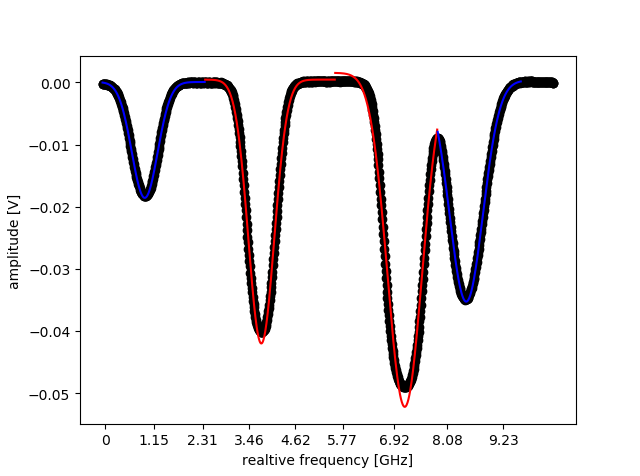
\includegraphics[width=0.7\textwidth]{Verbesserung/plot_fit_iso.png}
    \caption{Fit of the Gauss-curves; Red: ($^{85}$Rb), Blue: ($^{87}$Rb)}
\end{figure}\\
Now we calculate the integral over the gaussian curves:
\begin{equation}
    \int_{-\infty}^\infty -a\cdot\exp\left(\frac{-(x-b)^2}{2c^2}\right)=a\sqrt{2\pi c^2}
\end{equation}\newpage
It follows:
\begin{table}[h]
    \centering\begin{tabular}{c|c}
        Dip & Area\\\hline
        1 ($^{87}$Rb)&0,013302\\
        2 ($^{85}$Rb)&0,063096\\
        3 ($^{85}$Rb)&0,099945\\
        4 ($^{87}$Rb)&0,064184
    \end{tabular}
    \caption{Areas of the dips}
\end{table}\\
Now the individually Areas of the corresponding isotopes are summed up and divides throug the whole area:
\begin{table}[h]
    \centering\begin{tabular}{c|cc}
        Isotope & measured & theoretical\\\hline
        ($^{85}$Rb)&0,6778&0,7217\\
        ($^{87}$Rb)&0,3222&0,2783
    \end{tabular}
    \caption{Distribution of the isotopes}
\end{table}\\
The calculated values are close to the theoretical ones.
The difference is about 5\%.\newpage
\section{Doppler free signal}
\subsection{Doppler free signal of the absorptiondips}
Here are the Doppler-free signals of the absorption dips.
We used here the balanced channel:
\begin{figure}[h]
    \centering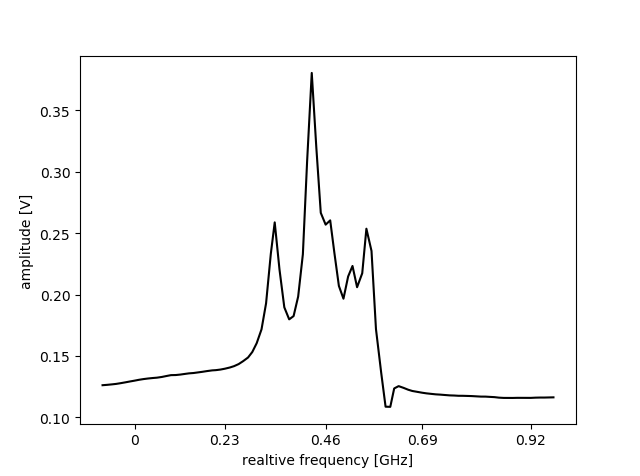
\includegraphics[width=0.6\textwidth]{Verbesserung/plot_peak1.png}
    \caption{First dip in the whole spectrum}
\end{figure}
\begin{figure}[h]
    \centering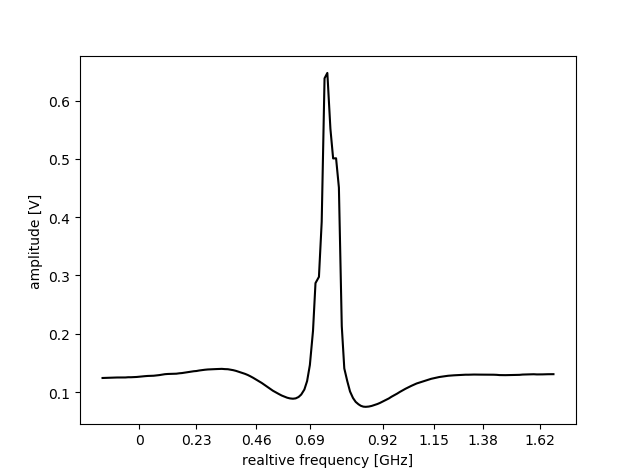
\includegraphics[width=0.6\textwidth]{Verbesserung/plot_peak2.png}
    \caption{Second dip in the whole spectrum}
\end{figure}
\begin{figure}[h]
    \centering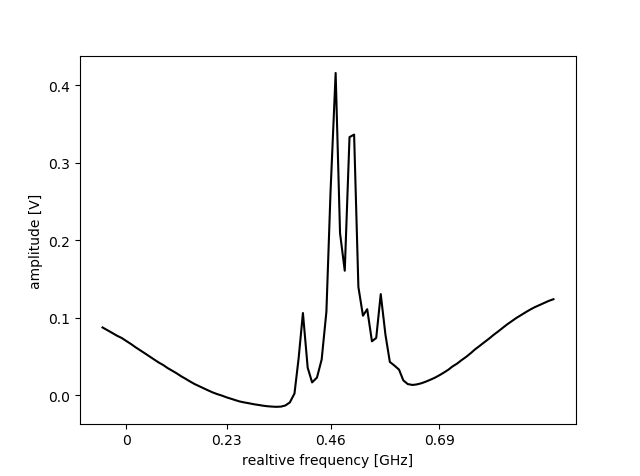
\includegraphics[width=0.6\textwidth]{Verbesserung/plot_peak3.png}
    \caption{Third dip in the whole spectrum}
\end{figure}
\begin{figure}[h]
    \centering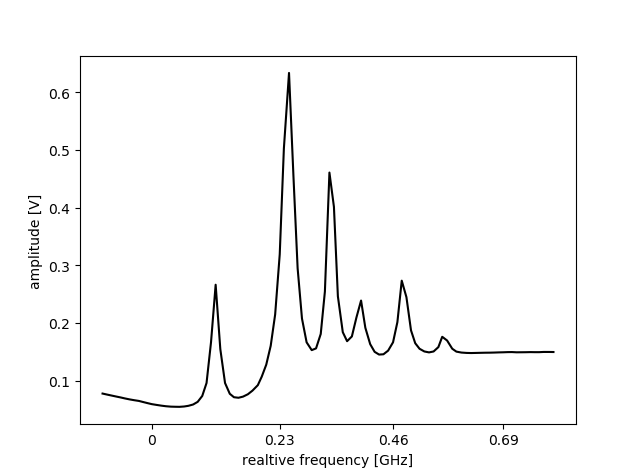
\includegraphics[width=0.6\textwidth]{Verbesserung/plot_peak4.png}
    \caption{Fourth dip in the whole spectrum}
\end{figure}\newpage
\subsection{Fitting of the Lorentz-profile}
At first we select one measurment of one peak (in our case peak number one) of the spectrum.
Then we seperate the data of the peak to each dip and fit a lorentz-profile to it.
The lorentz-profile is defined as \citep[][]{Lorentzkurve-Wiki}:
\begin{equation}
    f(x)=\frac{a\cdot b}{(x-b)^2+c^2}+d
\end{equation}
Where $a$ is the amplitude, $b$ the maximum, $c$ the width of the peak and $d$ the shift on the y-axis.\\
Then we fit the lorentz-profile to each dip of one peak.\newpage
After it the result looks like this:
\begin{figure}[h]
    \centering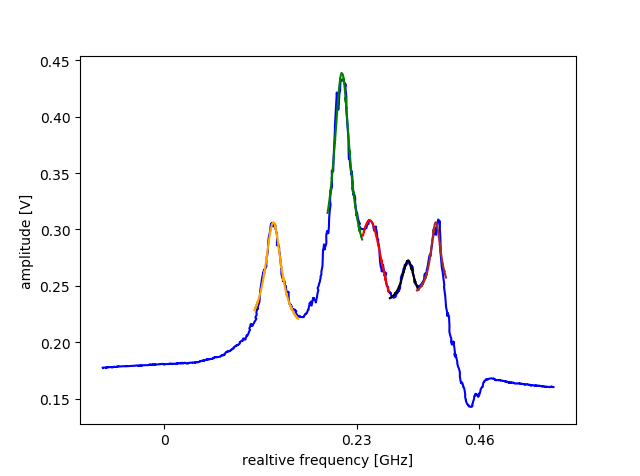
\includegraphics[width=0.7\textwidth]{Verbesserung/plot_einzelne_peaks.png}
    \caption{Peak No.1 with the lorentz-fit}
\end{figure}\\
Here is a table with the resulting variables:
\begin{table}[h]
    \centering\begin{tabular}{c|cccc}
        Dip & $a$ & $b$ & $c$ & $d$\\\hline
        1 &0,31&141,88&0,45&0,18\\
        2 &0,42&142,05&0,09&0,30\\
        3 &0,31&142,13&0,05&0,24\\
        4 &0,27&142,23&0,11&0,25\\
        5 &0,31&142,30&0,21&0,14
    \end{tabular}
    \caption{Fitting parameters of the lorentz fit}
\end{table}\\
In the plot are smaller and larger dips.
Ther larger dips are likely coming from 'Cross-over signals'.\\

To determine the energetic distance between the tops of two dips, we use the conversion of the current into wavelength:
\begin{equation}
    \Delta E_{i,i+1}=\frac{hc}{\lambda_{i+1}}-\frac{hc}{\lambda_{i}}=hc\left(\frac{1}{\lambda_{i+1}}-\frac{1}{\lambda_{i}}\right)
\end{equation}
To convert current into wavelength we fit a line to the current-wavelength correspendentive and get:
\begin{equation}
    \text{wavelength} = 1,3\cdot10^{-3}\cdot\text{current}+780,063
\end{equation}\newpage
So we get:
\begin{table}[h]
    \centering\begin{tabular}{c|c}
        Dip (i)& $\lambda$ (nm)\\\hline
        1&$780,247444\pm0,000013$\\
        2&$780,247665\pm0,000013$\\
        3&$780,247769\pm0,000013$\\
        4&$780,247899\pm0,000013$\\
        5&$780,247990\pm0,000013$
    \end{tabular}
    \caption{Wavelength of the dips}
\end{table}\\
And for the distance
\begin{table}[h]
    \centering\begin{tabular}{c|cc}
        Dip (i$\to$i+1)& $\Delta E_{i,i+1}$ ($10^{-26}\,$J)& $\Delta \nu_{i,i+1}$ (MHz)\\\hline
        1$to$2 &$7,2111\pm0,59989$&$108,8298\pm9,0534$\\
        2$to$3 &$3,3935\pm0,59989$&$51,21404\pm9,0532$\\
        3$to$4 &$4,2418\pm0,59989$&$64,01753\pm9,0534$\\
        4$to$5 &$2,9693\pm0,59989$&$44,81225\pm9,0534$
    \end{tabular}
    \caption{Energetic distances of the dips}
\end{table}\\
If you look now into the datasheet of the 85-Rb line \citep[][]{AnhangA}, you can see that two transitions are 'perfectly' measured.
The transition 2$\to$3 and 4$\to$5 are most likely Cross-over signals.\\

If you now compare both lines you get:
\begin{table}[h]
    \centering\begin{tabular}{c|cc}
        F-transition&$\Delta \nu_{meas.}$ (MHz) & $\Delta \nu_{theo.}$ (MHz) \\\hline
        4$\to$3 &$108,8298\pm9,0534$&120,640\\
        3$\to$2 &$64,01753\pm9,0534$ & 63,401
    \end{tabular}
    \caption{Comparism of experiment and theory}
\end{table}\\
You can see our measured values are similar to the theoretical values \citep[][]{AnhangA}.\\

If we use the FPI to calculate the frequency distances, first we measure the mean width of one period of the FPI:
\begin{align}
    \Delta T=\left(0,21\pm0,01\right)\,mA
\end{align}
For this we used the full measurment of all lines, because it has the most FPI-Peaks in it and the peaks themself are relative sharp and not noisy.\\
So the frequency distance per 'mA' is:
\begin{align}
    \Delta f&=\frac{\Delta x}{\Delta T}\cdot \Delta\nu_{FSR}\\
    \Delta f&=549,52\,\frac{MHz}{mA}\cdot \Delta x
\end{align}
Here is $\Delta x$ the distance between two dips of the peak.\\
For the error follows:
\begin{align}
    s_{\Delta f}&=\sqrt{\left(\frac{\partial \Delta f}{\partial \Delta x}\cdot s_{\Delta x}\right)^2+\left(\frac{\partial \Delta f}{\partial \Delta T}\cdot s_{\Delta T}\right)^2+\left(\frac{\partial \Delta f}{\partial \Delta\nu_{FSR}}\cdot s_{\Delta\nu_{FSR}}\right)^2}\\
    s_{\Delta f}&=\sqrt{\left(\frac{s_{\Delta x}}{\Delta f}\cdot \Delta\nu_{FSR}\right)^2+\left(\frac{\Delta x}{\Delta T^2}\cdot s_{\Delta T}\cdot \Delta\nu_{FSR}\right)^2+\left(\frac{\Delta x}{\Delta f}\cdot s_{\Delta\nu_{FSR}}\right)^2}
\end{align}
We do it this way, because the distance between two peaks is less than one full period of the FPI.\\
With the fitted parameters (the position of the dips of the peaks) we can now calculate the frequency distances of the dips:
\begin{table}[h]
    \centering\begin{tabular}{c|cc}
        Dip (i$\to$i+1)&$\Delta \nu_{i,i+1}$ (MHz)\\\hline
        1$\to$2&$93,418\pm7,010$\\%0,17
        2$\to$3&$43,962\pm5,888$\\%0,08
        3$\to$4&$54,952\pm6,098$\\%0,10
        4$\to$5&$38,466\pm5,799$%0,07
    \end{tabular}
    \caption{frequency distances of the dips}
\end{table}\\
For the lines you now get:
\begin{table}[h]
    \centering\begin{tabular}{c|cc}
        F-transition&$\Delta \nu_{meas., FPI}$ (MHz) & $\Delta \nu_{theo.}$ (MHz) \\\hline
        4$\to$3 &$93,418\pm7,010$&120,640\\
        3$\to$2 &$54,952\pm6,098$ & 63,401
    \end{tabular}
    \caption{Comparism of experiment (with FPI) and theory}
\end{table}\\
As you see the values measured using the FPI are lower than the values that are calculated with the current-wavelength function.
The theoretical values are not covert by this values.
The reason of the difference can be, that we're using for the frequency distance per 'mA' the full measurment and not the measurment of the single line.
We're doing this, because the FPI is in the single-line measurment very noisy so its hard to count all of the peaks.
\newpage
\section{Hyperfineconstant}
The Hyperfineconstant $A$ is defined as \citep[][]{Kohler}:
\begin{equation}
    A = \frac{2\cdot\Delta E_{HFS}}{F(F+1)-J(J+1)-I(I+1)}
\end{equation}
Where $\Delta E_{HFS}$ is the distance between the hyperfine dips and the normal niveau.\\
We had not measured the normal niveau, so you can rewrite the definition of the Hyperfineconstant as the following:
\begin{equation}
    A = \frac{2\cdot\left(\Delta E_{1,2}\right)}{F_1(F_1+1)-F_2(F_2+1)}=\frac{2h\cdot\left(\Delta \nu_{1,2}\right)}{F_1(F_1+1)-F_2(F_2+1)}
\end{equation}
Here is $\Delta E_{1,2}/\Delta\nu_{1,2}$ the distance between the hyperfine dip 1 and 2.

For our transitions you get:
\begin{table}[h]
    \centering\begin{tabular}{c|c}
        F-transition&$A_{meas.}$ ($10^{-26}\,$J)\\\hline
        4$\to$3 &$1,80278\pm0,14997$\\
        3$\to$2 &$1,41395\pm0,19996$\\
    \end{tabular}
    \caption{Hyperfineconstants for measured dips}
\end{table}\\
So you get a hyperfineconstant of:
\begin{equation}
    A_{meas.}=\left(1,608365\pm0,174965\right)\cdot10^{-26}\,\text{J}
\end{equation}
The theoretical value is given as \citep[][]{AnhangA}:
\begin{equation}
    A_{theo.}=1,65665\cdot10^{-26}\,\text{J}
\end{equation}
If you compare the two values, the theoretical value is in the errorrange of the measured value.\newpage
\section{Temperature of the probe}
Throug the doppler-shift the width (\textit{full width, half maximum}) of one line gets expanded like \citep[][]{Wiki-Dopp}:
\begin{equation}
    f'=\frac{x_0}{c}\sqrt{\frac{k_B\cdot T}{m}}
\end{equation}
Where $f'$ is the shifted width, $x_0$ the maximum, $k_B$ the Boltzmann-constant, $m$ the Mass of the particle and $T$ the Temperature.\\
If we want the new FWHM:
\begin{equation}
    FWHM'=\frac{x_0}{c}\sqrt{8\ln(2)\frac{k_B\cdot T}{m}}
\end{equation}
We also know the FWHM for an gaussian-curve:
\begin{equation}
    FWHM=\sqrt{8\ln(2)}\cdot\sigma
\end{equation}
So the Temperature for the gas is calculated as:
\begin{equation}
    T=\frac{m}{k_B}\cdot\left(\frac{\sigma}{x_0}c\right)^2
\end{equation}
To calculate the speed of the particles, we presume it is boltzman-distributed:
\begin{align}
    \bar{v}&=\sqrt{\frac{8k_BT}{\pi m}}&\hat{v}&=\sqrt{\frac{2k_BT}{m}}
\end{align}
Where $\bar{v}$ is the average and $\hat{v}$ the most likely velocity.\\

So to each first dip of the absorption spectrum the gaussian-curve is fitted and the Temperature and velocitys are calculated:
\begin{table}[h]
    \centering\begin{tabular}{c||cc|ccc}
        $T_{real}$ (K)& $\bar{v}_{real}$ (m/s)& $\hat{v}_{real}$ (m/s)& $T_{calc}$ (K)& $\bar{v}_{calc}$ (m/s)& $\hat{v}_{calc}$(m/s)\\\hline
        296,55&271,8&170,3&331,73&287,4&254,8\\
        310,95&278,3&246,6&654,71&403,8&357,9\\
        329,15&286,3&253,8&802,83&557,2&396,3\\
    \end{tabular}
\end{table}\\
The real values (Temperature measured over the heater unit) and the calculated values differ a lot.
The first value is in comparism to the others quite good, but we have no clue, why the distance between the measured and calculated temperatur is growing.